\chapter{Experiments}

\section{AE vs VAE}

Our main goal is to create an end-to-end RL algorithm composed of an encoder followed by SAC. To determine wheter to use an AutoEncoder or a Variational AutoEncoder we investigate if the stochasticity of VAEs can help in learning a good representation of the actual state. In order to do so, we follow a simple approach, train multiples both AEs and VAEs to compare how much information they are able to recover on average from the latent vectors with an MSE loss. As described above, we run a single pre-train on the dataset and then the chosen encoder remains unchanged for the entire duration of the RL agent training. However, there are several choices that must be made before proceeding with the RL training, i.e. the size of the latent vector $z$ and wheter to use image augmentation or not to improve the robustness of our learned representation. In particular, we consider several augmentation techniques are randomly applied during the training, i.e. Gaussian and motion blurring, contrast normalization, additive Gaussian noise, sharpening and coarse dropout. In particular we consider an AE and a VAE neural network composed as respectively described in Listings \ref{lst:aenet} and \ref{lst:vaenet}. Each encoder has been trained three times for 50 epochs and with an early stopping on the fifth contiguos epoch with no improvement on the validation loss. After the training, each model is evaluated on the test set and the results are averaged and reported in Tables \ref{tab:aesim}-\ref{tab:vaereal}. The focus is mainly on the reconstruction loss mean since it describes which model maintains more information about original images from which the RL agent would benefit from. The standard deviation is also useful in understanding how consistent it is through the test set. Furthermore, in all cases the encoder reaches lower reconstruction loss mean when augmentation is disabled since its activation causes early stopping in all tested case. A further contribution to the reduction of the loss is given by a bigger latent vector, in fact in all cases the encoder with a latent space of 64 dimension performs better. Finally, our VAEs outperform significantly all the AEs, that is why we will use them to carry out all the next experiments, both in real world and in simulation. In Figures \ref{fig:realvaeexample} and \ref{fig:simvaeexample} is shown an example of what are the capabilities of the chosen VAEs in terms of reconstruction. From now on we will refer to the VAE trained on the dataset of pictures collected in the simulator with the name \textit{simulated VAE} and to the one trained on pictures collected in the real world with name \textit{real VAE} for simplicity. 


\begin{figure}[h]
  \begin{minipage}{.50\textwidth}
    \centering
    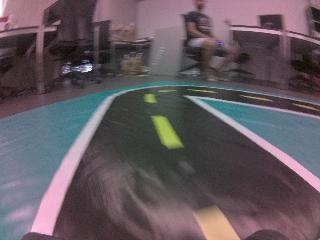
\includegraphics[height=0.50\textwidth]{experiments/11296.jpg}
  \end{minipage}%
  \begin{minipage}{.50\textwidth}
      \centering
      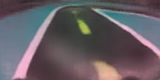
\includegraphics[width=0.60\textwidth]{experiments/11296.png}
  \end{minipage}
  \captionof{figure}{On the left an image from the real world as seen by the DonkeyCar camera, on the right the encoded and reconstructed image by the chosen VAE with a reconstruction loss of 112.}
  \label{fig:realvaeexample}
\end{figure}
\begin{figure}
  \begin{minipage}{.50\textwidth}
    \centering
    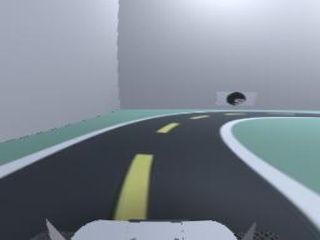
\includegraphics[height=0.50\textwidth]{experiments/1160.jpg}
  \end{minipage}%
  \begin{minipage}{.50\textwidth}
      \centering
      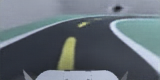
\includegraphics[width=0.60\textwidth]{experiments/1160.png}
  \end{minipage}
  \captionof{figure}{On the left an image from the simulator as seen by the DonkeyCar camera, on the right the encoded and reconstructed image by the chosen VAE with a reconstruction loss of 17}
  \label{fig:simvaeexample}
\end{figure}

\begin{table}
  \centering
  \begin{tabular}{|c|c||c|c|c|c|}
  \hline
  Z\_SIZE & AUGMENTATION & MEAN & STD & MAX & MIN \\ \hline
  \multirow{2}{*}{32} & False & 121.54 & 102.42 & 795.44 & 45.61 \\
  & True & 164.57 & 95.51 & 783.03 & 65.13  \\ \hline
  \multirow{2}{*}{64} & False & 103.54 & 79.14 & 588.14 & 40.84 \\
  & True & 137.24 & 74,02 & 611,81 & 63,05  \\ \hline
  \end{tabular}
  \caption{AE trained in simulation - reconstruction loss}
  \label{tab:aesim}

  \begin{tabular}{|c|c||c|c|c|c|}
  \hline
  Z\_SIZE & AUGMENTATION & MEAN & STD & MAX & MIN \\ \hline
  \multirow{2}{*}{32} & False & 377.07 & 87.53 & 756.7 & 239.46 \\
  & True & 493.84 & 99.40 & 807.67 & 289.99  \\ \hline
  \multirow{2}{*}{64} & False & 311.1 & 78.5 & 695.65 & 177.77 \\
  & True & 411.37 & 77.30 & 647.68 & 241.87 \\ \hline
  \end{tabular}
  \caption{AE trained in real world - reconstruction loss}
  \label{tab:aereal}

  \begin{tabular}{|c|c||c|c|c|c|}
  \hline
  Z\_SIZE & AUGMENTATION & MEAN & STD & MAX & MIN \\ \hline
  \multirow{2}{*}{32} & False & 59.1 & 60.41 & 620.93 & 18.88 \\
  & True & 116.31 & 71.11 & 771.88 & 51.10  \\ \hline
  \multirow{2}{*}{64} & False & 45.15 & 43.49 & 480.22 & 14.34 \\
  & True & 112.17 & 59.79 & 573.19 & 54.28  \\ \hline
  \end{tabular}
  \caption{VAE trained in simulation - reconstruction loss}
  \label{tab:vaesim}

  \begin{tabular}{|c|c||c|c|c|c|}
  \hline
  Z\_SIZE & AUGMENTATION & MEAN & STD & MAX & MIN \\ \hline
  \multirow{2}{*}{32} & False & 227.4 & 44.74 & 418.7 & 140.12 \\
  & True & 263.87 & 52.29 & 478.26 & 172.70 \\ \hline
  \multirow{2}{*}{64} & False & 184.56 & 36.86 & 347.59 & 96.7 \\
  & True & 230.66 & 42.24 & 402.67 & 156.61  \\ \hline
  \end{tabular}
  \caption{VAE trained in real world - reconstruction loss}
  \label{tab:vaereal}
\end{table}


\begin{center}
    \begin{minipage}{0.9\linewidth}
      \lstinputlisting[caption=AE network, label=lst:aenet]{ae.txt}
      \end{minipage}
    \begin{minipage}{0.9\linewidth}
      \lstinputlisting[caption=VAE network, label=lst:vaenet]{vae.txt}
      \end{minipage}
\end{center}

\section{RL algorithm}

\subsection{Reward function}
Designing a reward function that can work on both simulated and real environments is not trivial given the fundamental differencences between them. In simulation, for example, the environment can provide a supervision and a set of useful information, i.e. the position of the car and the speed. In our real setup, instead, the DonkeyCar can only leverage information coming thrugh the camera frames. The reward function designed to work in simulation consists of four parts. The first one is a single point gained  by the agent for every step made, with the goal of improving the length of the path as much as possible. Secondly, a throttle reward term increases the reward by a value proportional to the throttle so as to encourage the agent to drive as fast as possible. Moreover, a cross track error penalty is a proportial to the distance of car from the center of the roadway that disincentive the penalizes the agent as soon as it moves away from the center. Finally, as soon as the agent crashes or exceed the maximum cross track error a big penalty is given. Thus, the reward function to be maximized is composed as follow:

\begin{equation}
  \label{eq:stdreward}
    r_t = 1 + throttle\_reward + cte\_penalty + \left\{\begin{matrix}
    if done & crash\_error \\ 
    else & 0  
    \end{matrix}\right.
\end{equation}
In our setup, the throttle is kept constant for the purposes of this thesis.
The reward function described above is used to test our simulated algorithm and as a starting point, however, we need to adapt it such that it can work also in real world. To tackle the issue we simply remove the CTE penalty, eventhough this will lead to a major problem described in the next section. The final reward function that has proven to work in both environments and we use in our trainings is computed as:
\begin{equation}
  \label{eq:realreward}
    r_t = 1 + throttle\_reward + \left\{\begin{matrix}
    if done & crash\_error \\ 
    else & 0  
    \end{matrix}\right.
\end{equation}
Since we want the real and the simulated version of our agent as similar as possibile Equation \ref{eq:realreward} is used in both cases.

\subsection{Training the simulated RL agent}
As a baseline for RL algorithm we used the source code provided by \citet{DBLP:journals/corr/abs-2008-00715}. Their algorithm allows both simulated and real training, however training on simulation with communication being over-the-internet is more computationally expensive and more prone to errors. Thus, for the simulation, we refactor the algorithm such that the communication happens locally. Beside that, his algorithm uses an AE which need to be changed with the VAE chosen above. In order to train our agents, we need to define what is the best strategy in terms of starting point. We identified four main options, the first one let the agent start always at the starting line, in the second option it starts from a random checkpoint, in the third one it starts on the latest checkpoint reached in previous episode and finally the last option make it start from all checkpoint cyclically. Defining in simulation what it the best strategy can save computational time in real world training. To chose where the car should starts a new lap we trained 4 different model, one for each option aforementioned, in order to identify which one eventually converges more quickly and if it does. The quality measures to evaluate the trained agents, illustrated below in Figure \ref{fig:agentresults}, are the \textit{Episode success rate} that shows how many laps has been completed on average during the training, the \textit{Episode Reward mean} and the \textit{Episode Length mean}. All the model have been trained for 100k iterations which correspond to $\approx 2$ hours of training. \textit{ Agent 1} started each lap at a random checkpoint,\textit{ Agent 2} started always at the starting line,\textit{ Agent 3} at the latest checkpoint reached during the last episode and, finally,\textit{ Agent 4} cyclically uses all the checkpoints.
\begin{figure}[h]
  \centering
  \begin{subfigure}{.5\linewidth}
      \centering
      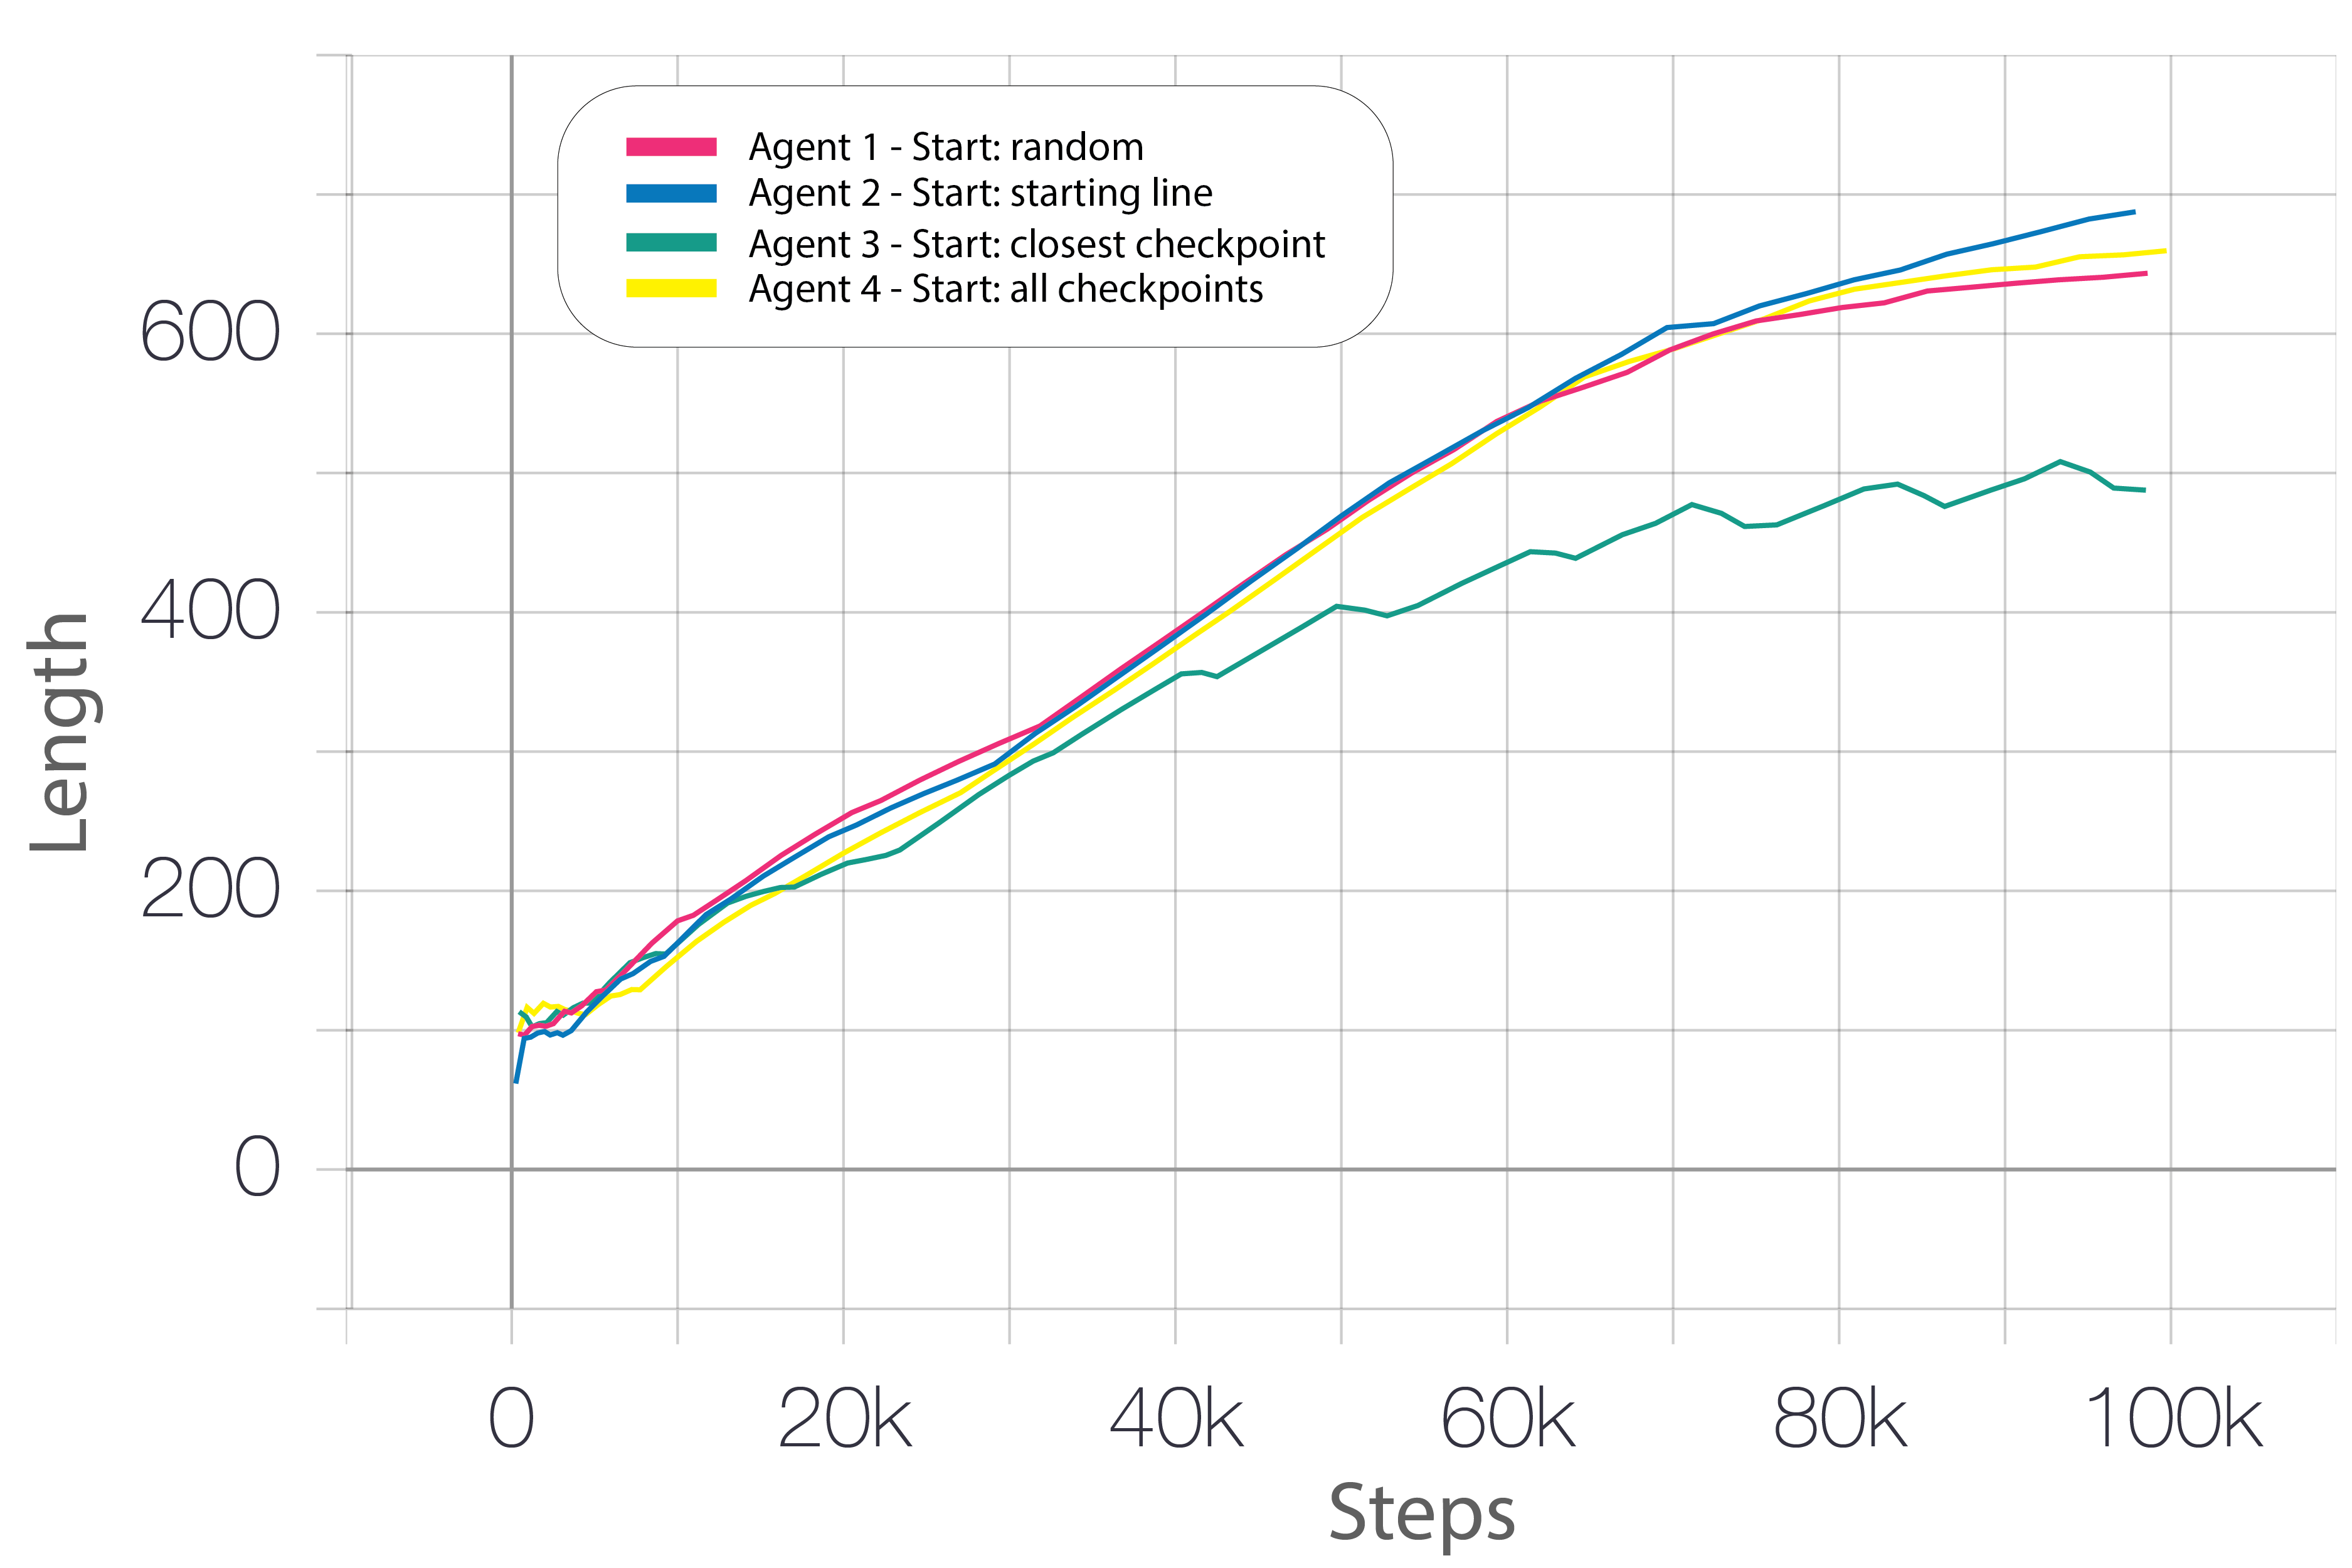
\includegraphics[width=1\textwidth]{experiments/len_mean.png}
      \caption{Episodes length mean}\label{fig:len}
  \end{subfigure}%
      \hfill
  \begin{subfigure}{.5\linewidth}
      \centering
      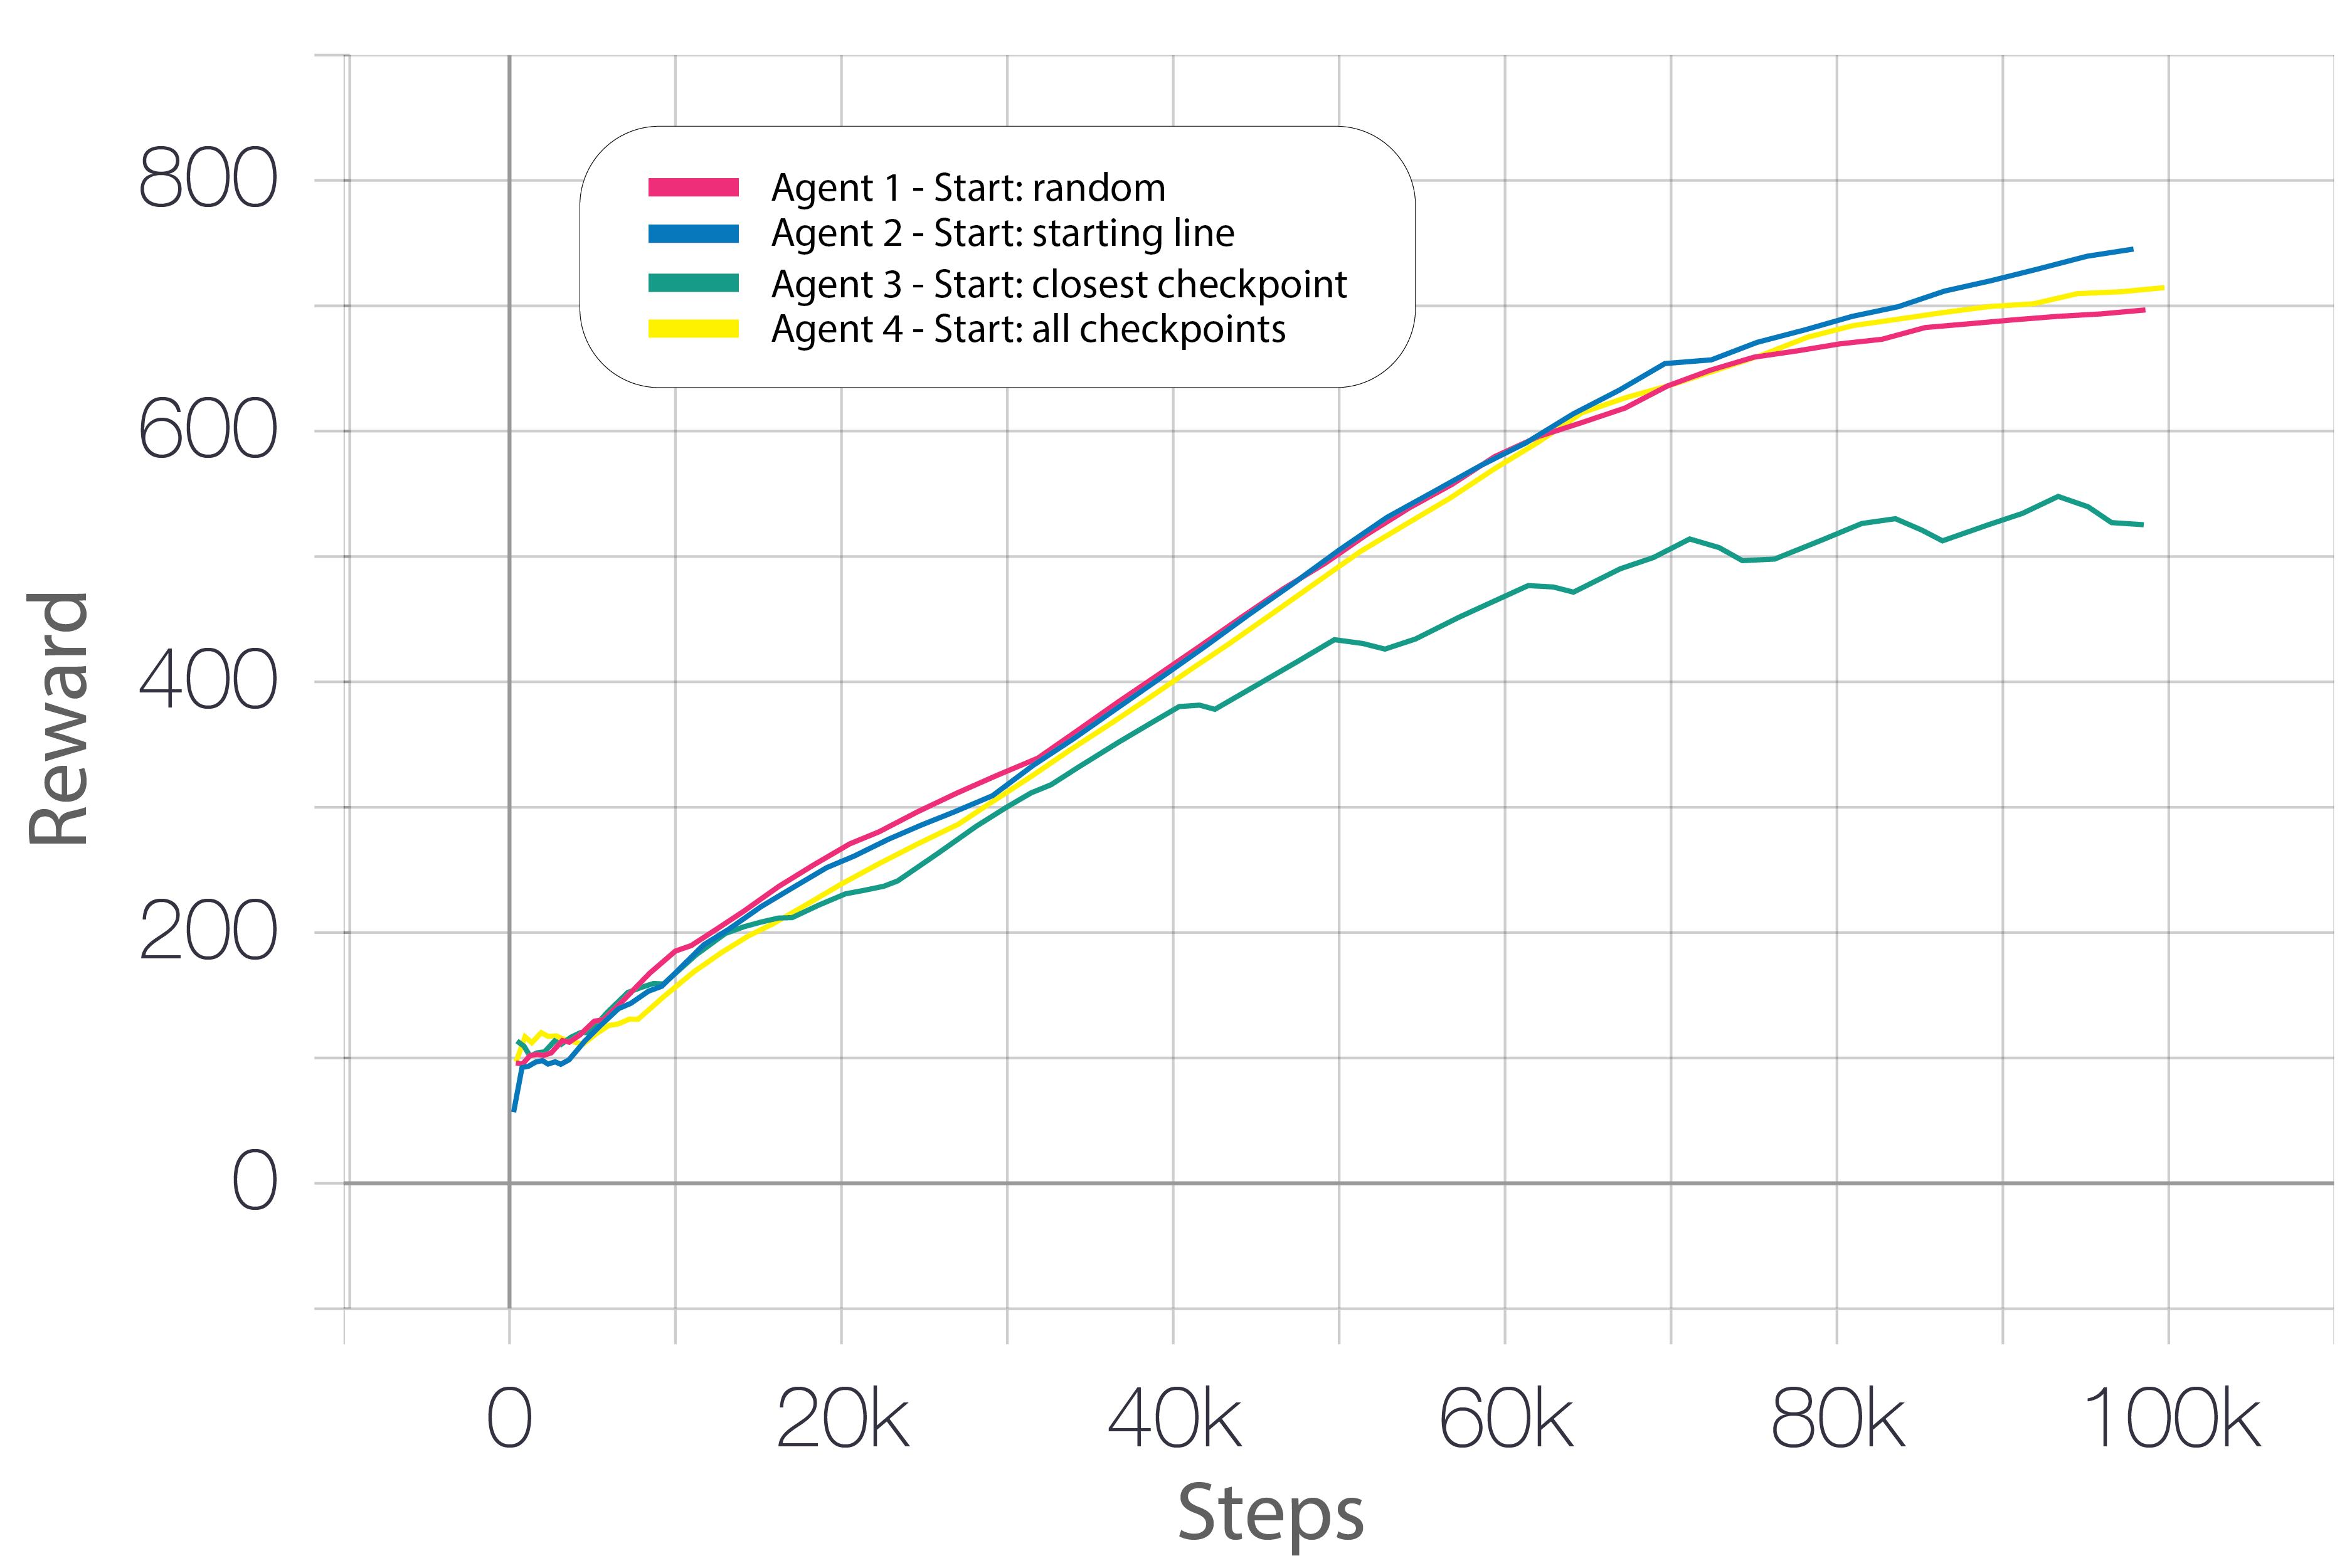
\includegraphics[width=1\textwidth]{experiments/rew_mean.png}
      \caption{Episodes reward mean}\label{fig:rew}
  \end{subfigure}
  
  \bigskip
  \begin{subfigure}{.5\linewidth}
    \centering
    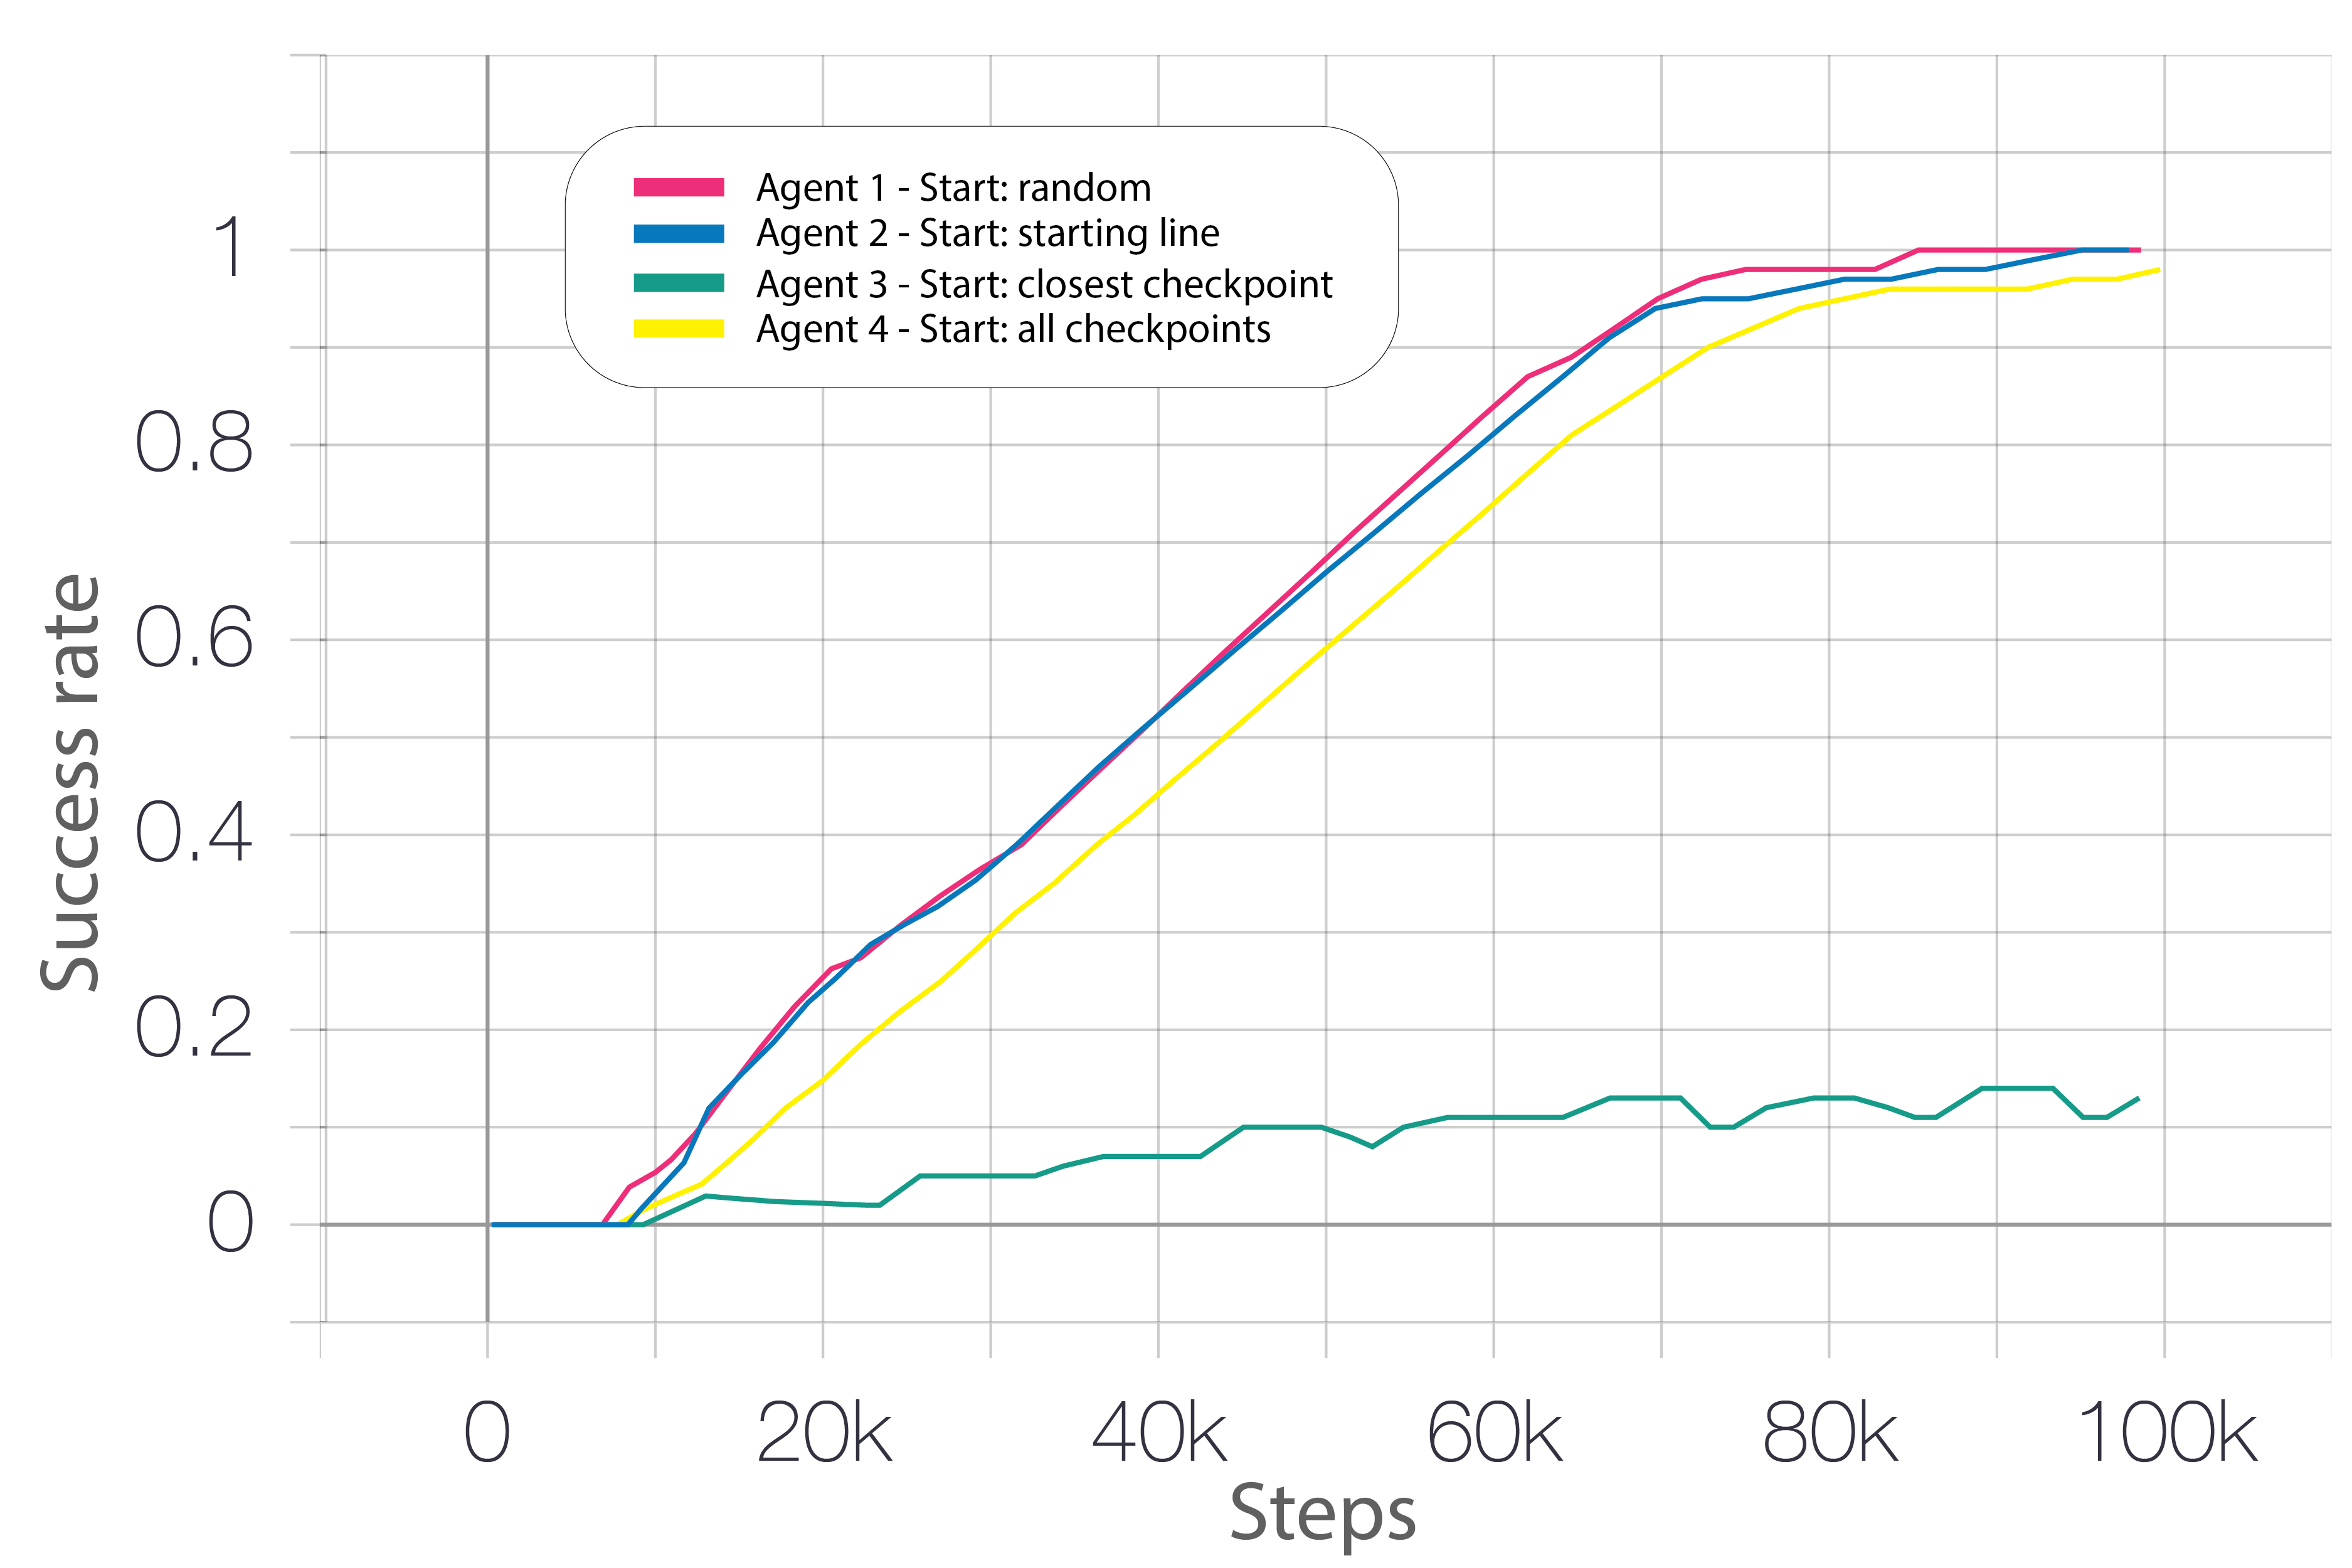
\includegraphics[width=1\textwidth]{experiments/success_mean.png}
    \caption{Success rate mean}\label{fig:succ}
  \end{subfigure} 
  \caption{Agents trained in simulation. Each agent has been trained with a different starting modality and has been trained for 100k steps.}
  \label{fig:agentresults}
\end{figure}
During our experiments we noted that, in the best case, a lap may takes $\approx 350$ iterations to be completed. The agents are all able to successfully learn to drive with a strict maximum CTE except for the agent that started new laps from the latest checkpoint. There are two interesting evidences that come out of those trainings. The first one is that even though the success rate mean approaches $100\%$, meaning that the agent is able to consistently finish laps, the reward mean keeps growing. This shows a limitation in the reward function used, in fact the agent gets a reward for every steps and hence it learns to finish the lap following the longest path it has discovered. Beside that, the best way to lengthen the path is a zig-zag behavior that allows also a doubling of the reward per lap. Secondly, the agent that start at the latest checkpoint keeps improving the reward up to more than an equivalent completed lap, however it never finishes a lap as described in Figure \ref{fig:succ}. The reason behind this strange behavior is that the agent found a bug in the simulator used, as shown in Figure \ref{fig:bug}. Essentially, there is a a little spot, off track, close to the steepest turn where the CTE is not is correctly detected and consequently the episode is not terminated. The fact this behavior happened only with this agent stands in the training modality. When the agent reach this checkpoint, he cannot easily reach the next checkpoint given the toughness of the turn, instead it finds much easier to explore the bugged spot which is almost right in front of it when it approaches the turn.

\begin{figure}[h]
  \begin{center}
    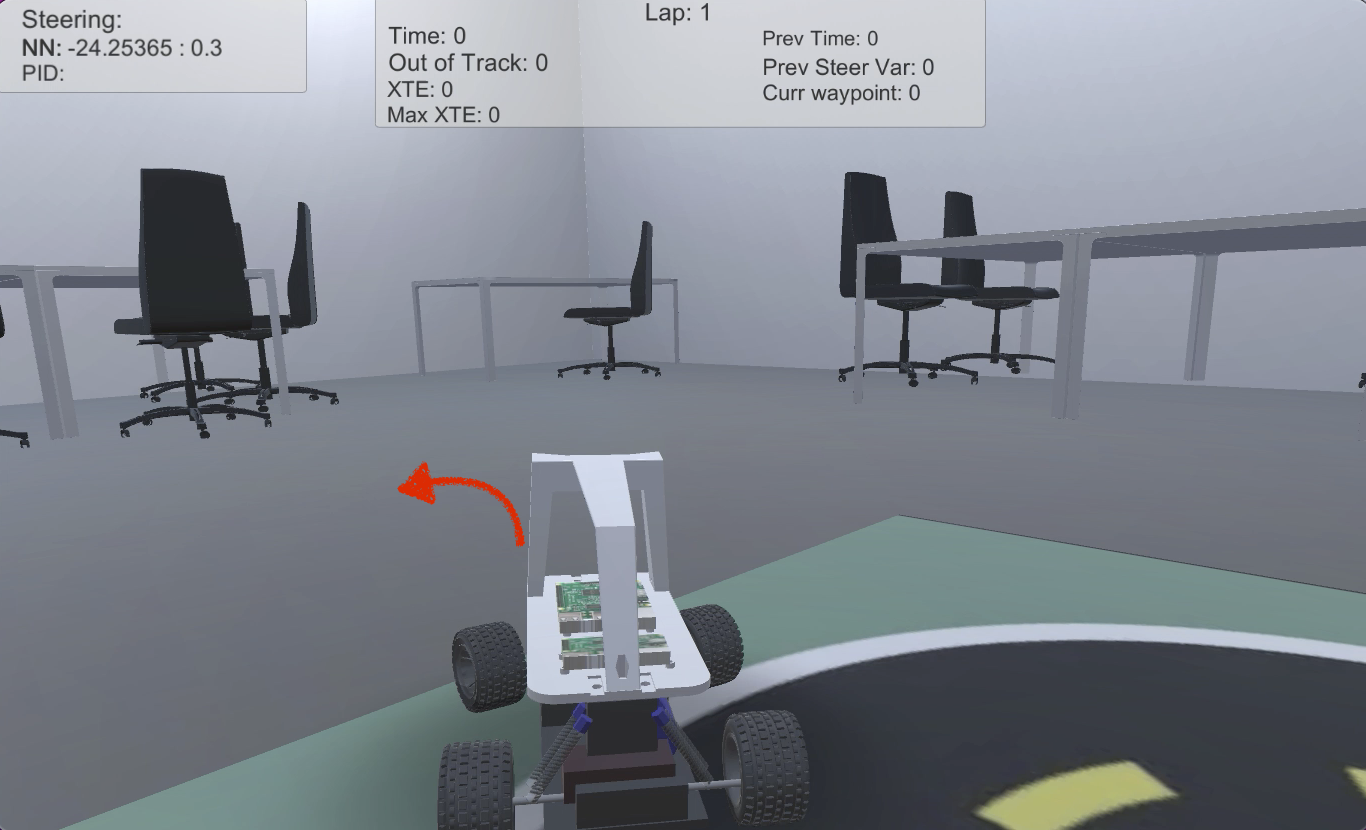
\includegraphics[width=0.50\textwidth]{experiments/bug.png}
  \end{center}
  \caption{Spotted bug in the simulator}
  \label{fig:bug}
\end{figure}

To further test the trained agents, for 10 laps it is measured how many times a lap has been completed, how many times the agents crashes, and finally how many time it exceed the roadway but is able to recover and finish the lap without crashing. The result are presented in Table \ref{tab:simagent}.
\begin{table}
  \centering
  \begin{tabular}{|c|c|c|c|c|c|}
  \hline
  AGENT & OOT & OBE & LAPS & AVG LENGTH & AVG REW \\ \hline
  1 & 0 & 0 & 10 & 595 & 644 \\
  2 & 0 & 4 & 10 & 599 & 647  \\ \hline
  3 & 0 & 0 & 10 & 624 & 676 \\
  4 & 10 & 29 & 0 & 460 & 495  \\ \hline
  \end{tabular}
  \caption{Agents results averaged over 10 laps. Out Of Track (OOT) measures crashes, Out of Bound Error measure how many times it exceed the max CTE, and finally LAPS counts the completed laps.}
  \label{tab:simagent}
\end{table}
Thus, excluding\textit{ Agent 4 }because of the simulator's bug, three agents learned to drive successfully and in most cases they always stay entirely on track without the need of any additional sensor and with the only problem of the shaky driving which is still acceptable for the purposes of this thesis, in most cases they never get out of track, and if they do they are able to recover consistently.

\subsection{Training the real RL agent}
In real world instead the source code provided by \citet{DBLP:journals/corr/abs-2008-00715} is kept untouched beside the encoder, with the main goal being to replicate their results but with a more performing VAE as resulted in our tests. Given that in real world the simulator supervision is not available, all the agents tested in previous section are good candidates to be used, also \textit{Agent 4} that cannot explore anymore the simulator's bug. However from the tests, it resulted that all the agents struggle to learn driving an entire lap in reasonable time, except\textit{ Agent 4 }that start his laps at the latest checkpoint reached in the last episode. Human supervision is about stopping the episode anytime the car exceeds the track boundaries with all 4 wheels, while the host machine automatically stops the car when it reaches 1000 steps ($\sim 2.5$ laps). In figure \ref{fig:realresult} are shown the performances in training. The laying of the car on the latest checkpoint has been intentionally approximate on the area close to the checkpoint. This brought a main advantage, the agent learns quicker since it is able to see the area in front of it from many points of view. It results useful when the car will start to cross many checkpoints per episode, since the direction from which the car arrives to a checkpoint can vary a lot, it has been trained to drive on many possibile trajectories and will join the various sections well. The overall training procedure results to be simple and fast ($\sim$ 30 minutes) to get an entire lap completed. In five to twenty episodes, the first two turn are learned decently. Most of the time is spent on the steepest turn. As shown in Figure \ref{fig:rlen}, the graph is characterized by ups and downs, as soon as the car starts at the starting line, it learns quickly, then, when the steepest curve is reached it struggle to overcome it and the when it enventually does the length start to increase again. The process is repeated until it is almost consistently able to finish a lap. As soon as the agent has learned the steepest turn, it generalizes well on following turn, in fact little time is spent on them.

\begin{figure}[h]
  \centering
  \begin{subfigure}{.5\linewidth}
      \centering
      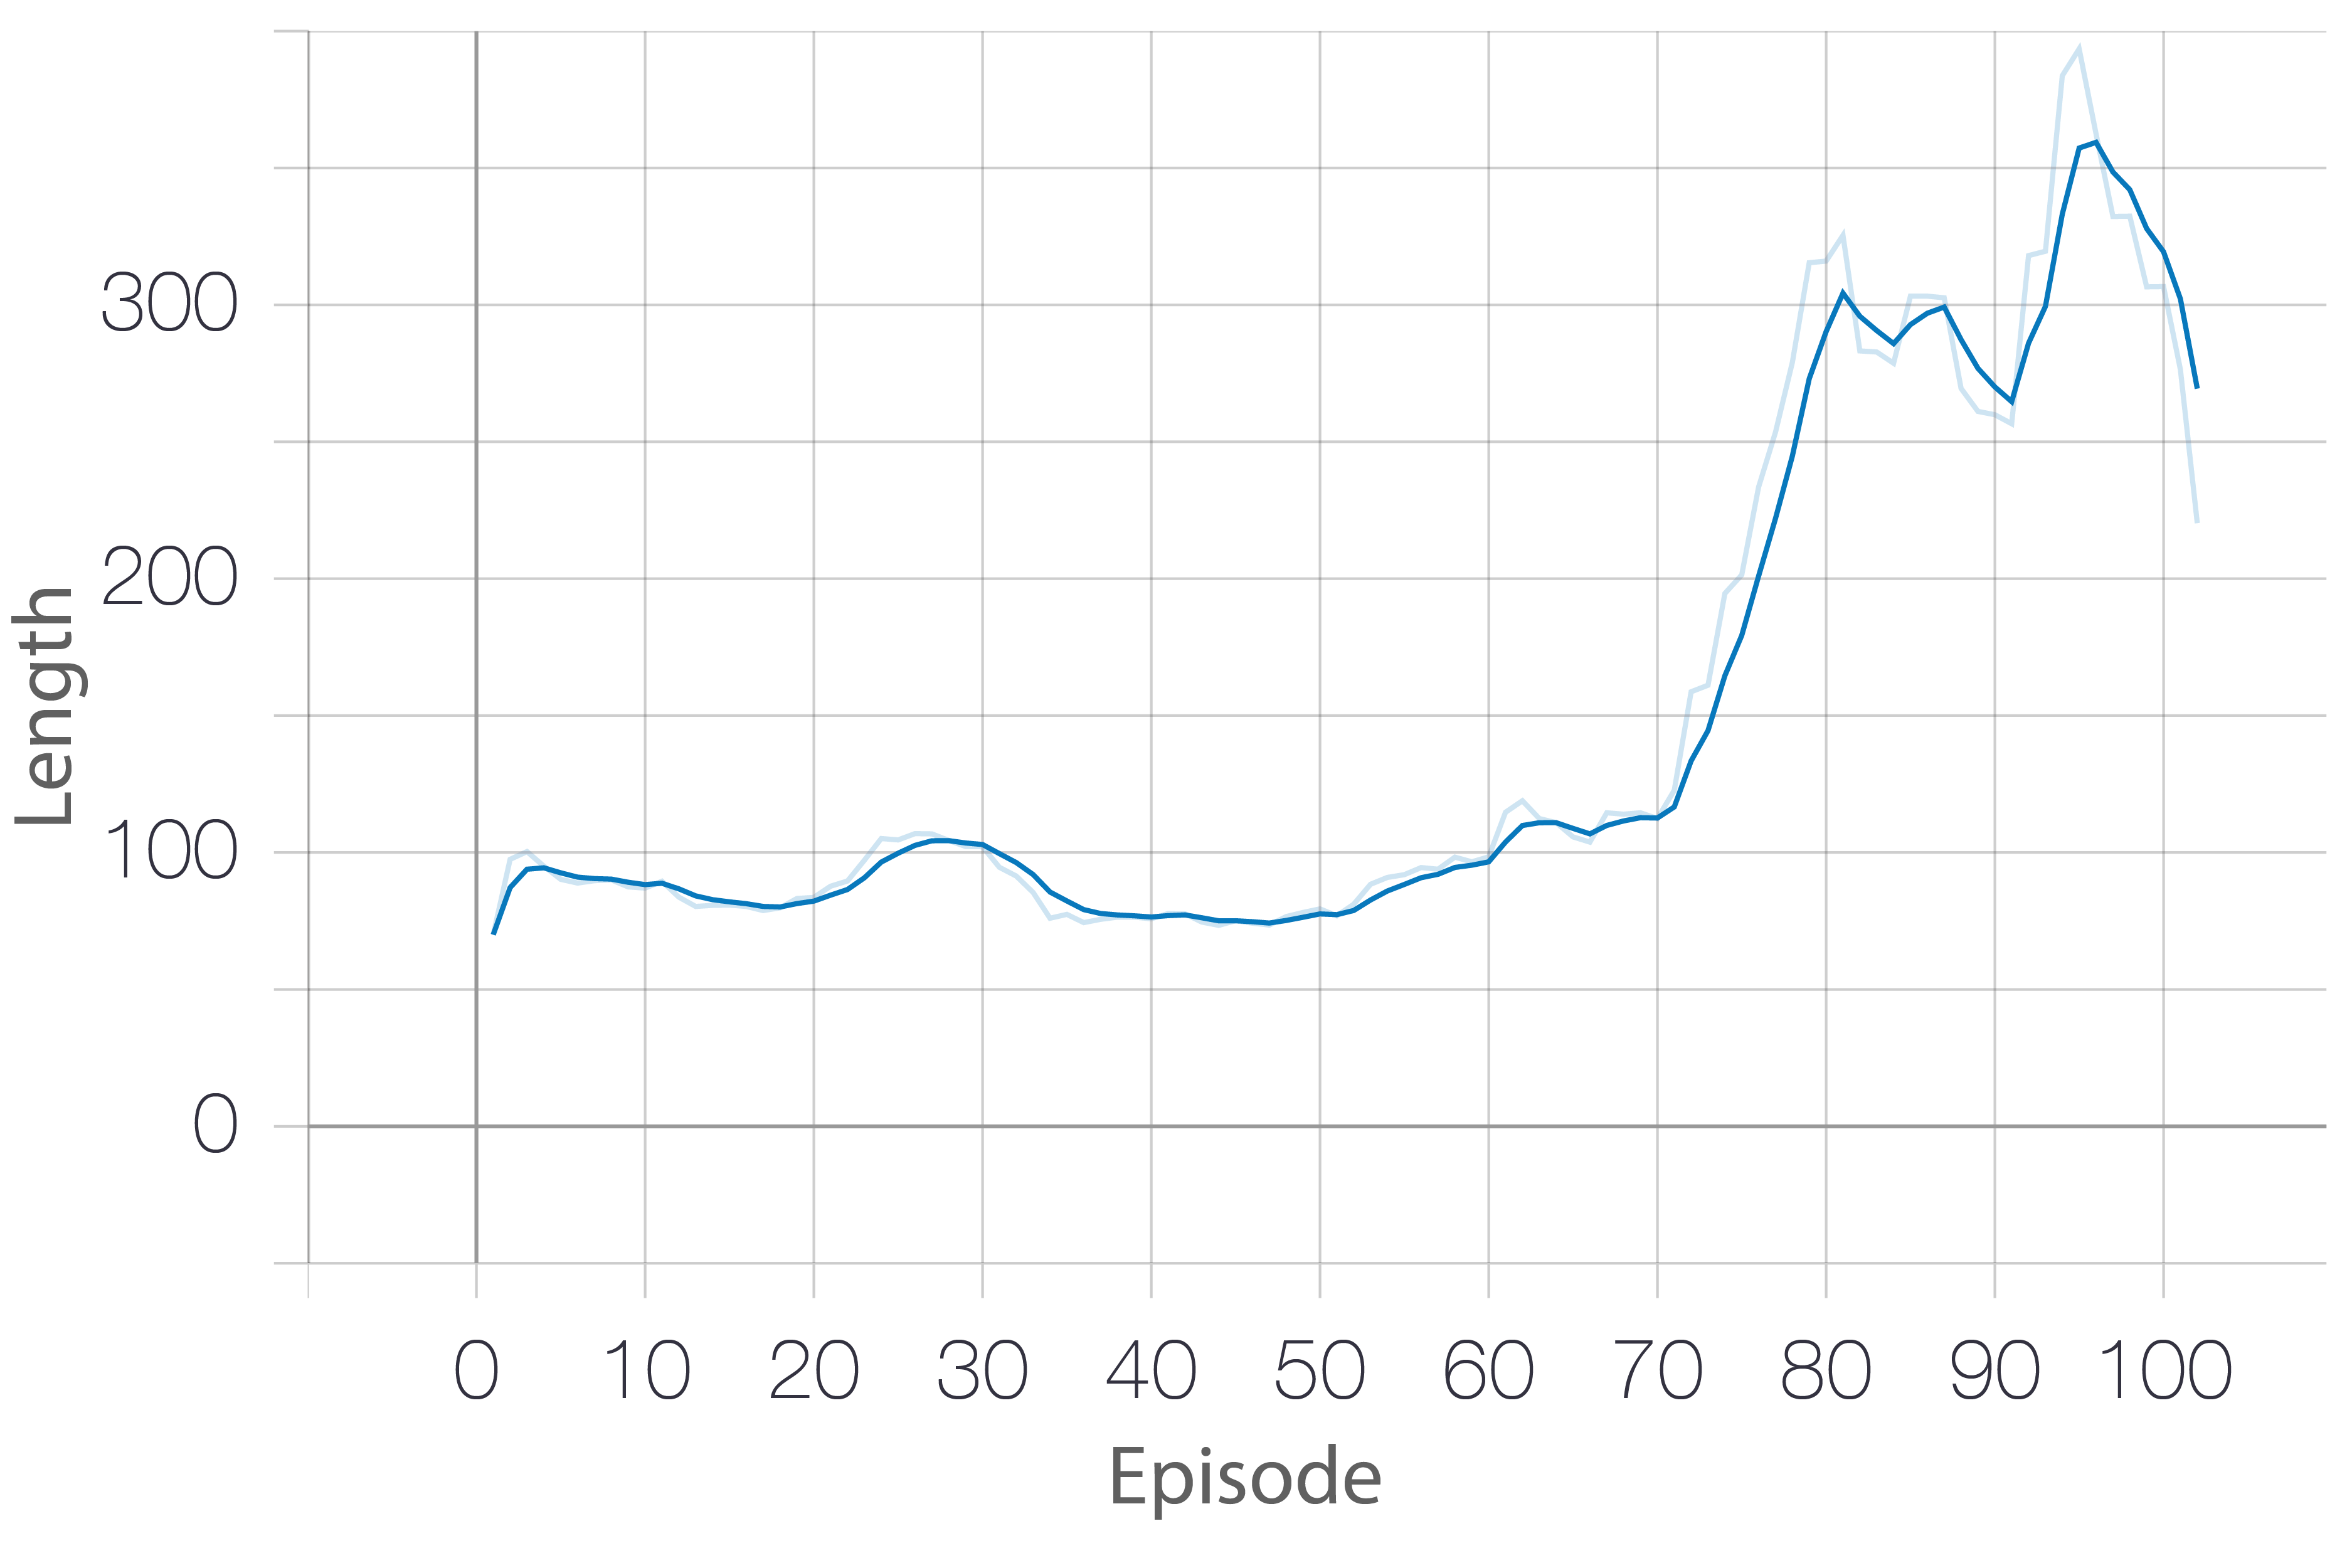
\includegraphics[width=1\textwidth]{experiments/real_len.png}
      \caption{Episodes length}\label{fig:rlen}
  \end{subfigure}%
      \hfill
  \begin{subfigure}{.5\linewidth}
      \centering
      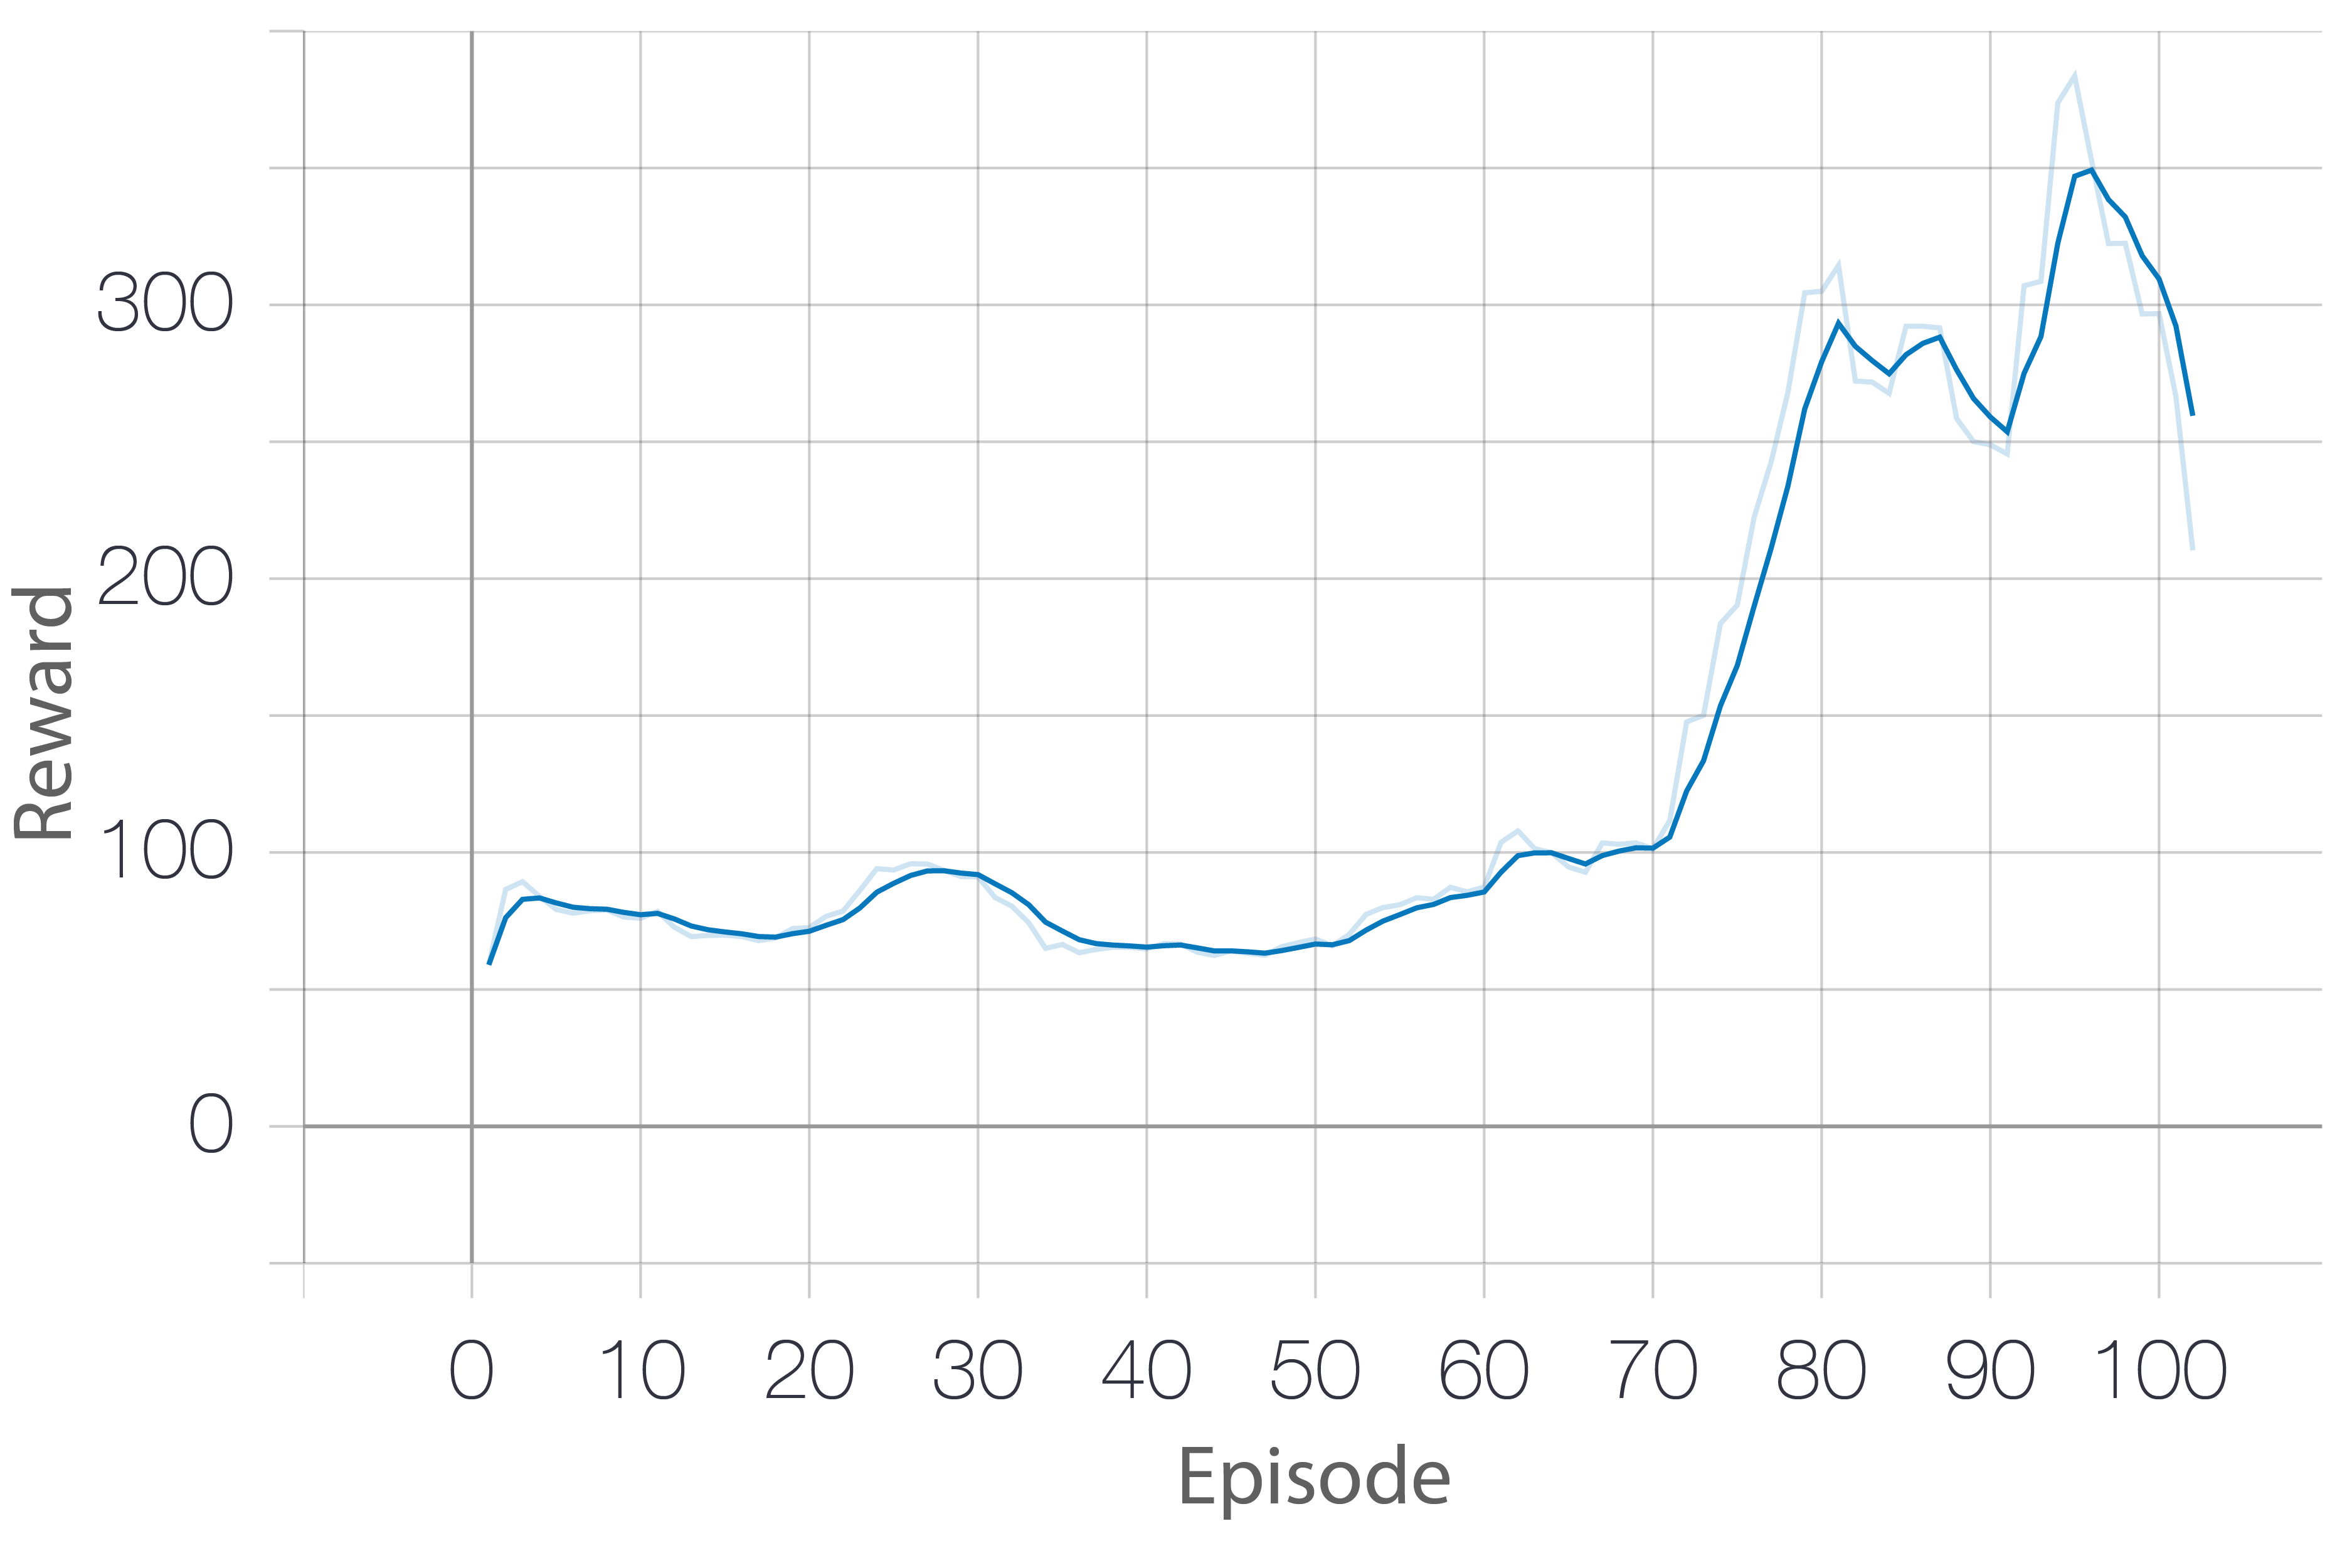
\includegraphics[width=1\textwidth]{experiments/real_rew.png}
      \caption{Episodes reward}\label{fig:rrew}
  \end{subfigure}
  \caption{Agent trained in real world starting each lap on the latest checkpoint}
  \label{fig:realresult}
\end{figure}

Unfortunately, in real world more metrics to measure the quality of the driving and to make comparisons with the simulated agents are not available. 

\section{Sim to Real}

In this sectin we present an unsuccessful attempt in driving our simulated DonkeyCar with the real agent trained above. SimToReal (S2R) and viceversa aims in deploying model trained in one environment to the other. In our case, since the real world environment, in our setup, does not provide enough metrics to benchmark our real world agent, we aim to make it works also in simulation. For example, in order to test the generalization of the real agent would be much easier in simulation where multiple tracks or obstacles can be implemented at a low cost. Another advantage brought by this approach is that an agent trained in simulation, can be moved into the real world and this would result in less expensive training procedures and eventually more robust agents. The idea is to pre-train a CycleGan \citep{CycleGAN2017} for image trasfiguration. In fact, the CycleGan is able to move an image into another domain keeping the original structure unaltered, but applying the style of the other domain as shown in Figure \ref{fig:cycleganexample}. Thus we leverage this property to transform images seen by the simulated camera of the DonkeyCar into what it would see in real world and viceversa. Then, a real agent will eventually be able to drive on the simulator since it does see pseudo-real images. On the other hand, in order to drive a real car with a simulated agent, our DonkeyCar has not enough computational power, hence it could not run in time a CycleGan, that has millions of parameters, to make the real car see pseudo-simulated images and drive with the simulated agent. However, the problem can be circumvented by training an agent entirely on simulation but with pseudo-real images. After training CycleGAN with our datasets, it is able to transfigure image with high fidelity as shown in Figure \ref{fig:cycleganexample}. In fact, in human eyes they are barely distinguishable. However, even if the result looks good it could not be the case for the autoencoder that needs to place similar real and pseudo real images close into the latent space and similarly for similar simulated and pseudo simulated images.

\begin{figure}[h]
  \centering
  \begin{subfigure}{.6\linewidth}
      \centering
      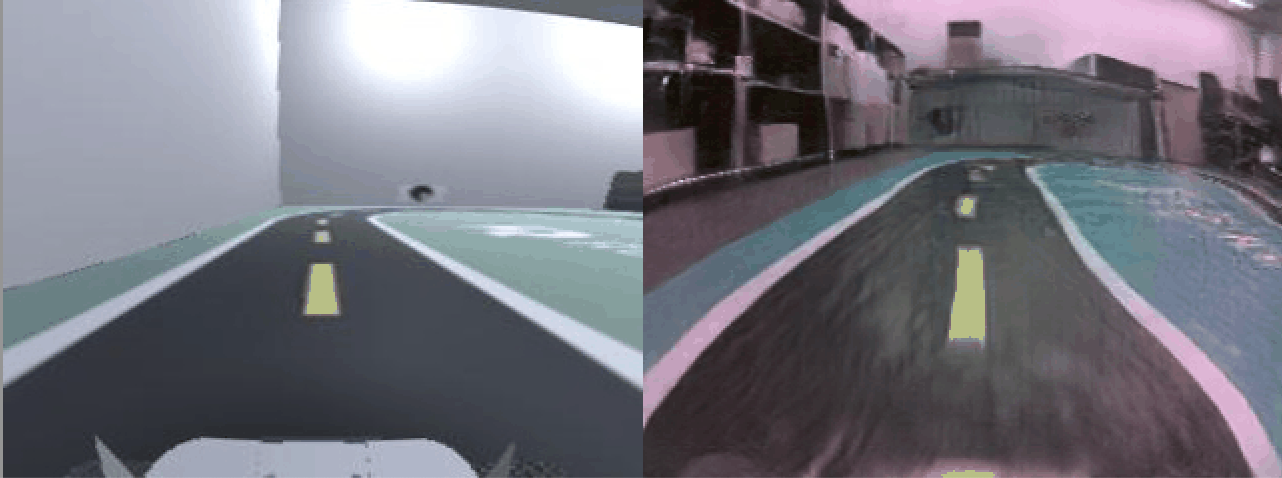
\includegraphics[width=1\textwidth]{experiments/s2r.png}
      \caption{From simulated images to pseudo-real}\label{fig:s2r}
  \end{subfigure}
      \hfill
  \begin{subfigure}{.6\linewidth}
      \centering
      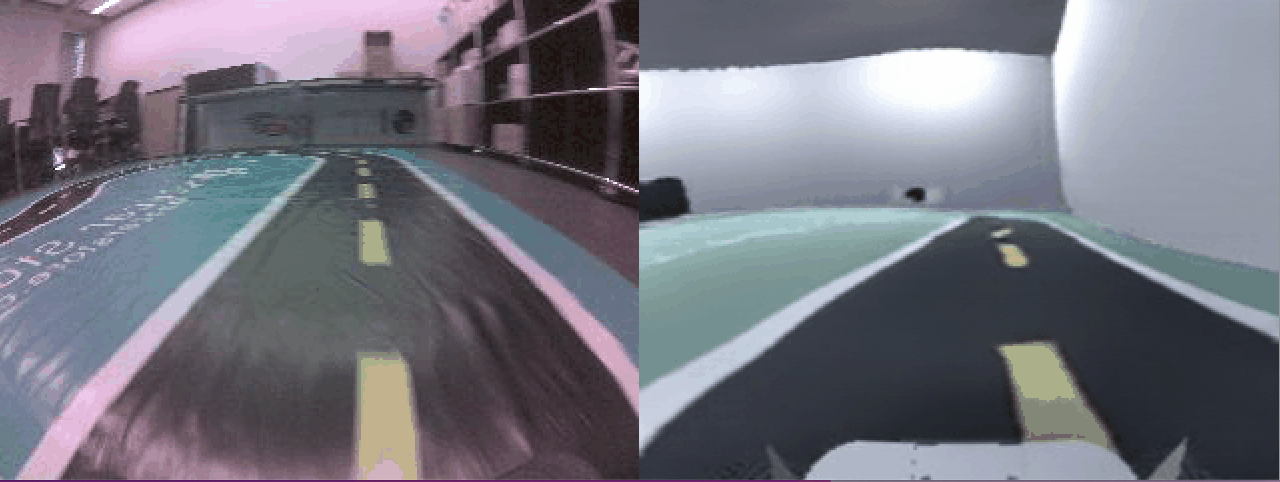
\includegraphics[width=1\textwidth]{experiments/r2s.png}
      \caption{From real images to pseudo-simulated}\label{fig:r2s}
  \end{subfigure}
  \caption{CycleGAN capabilities after training on our dataset}
  \label{fig:cycleganexample}
\end{figure}
Hence, the real test set is transformed through the CycleGAN and then forwarded through the real VAE chosen and similarly for the simulated test set. Given that 64 dimension cannot be visualized, a further dimensionality reduction is applied with t-SNE down to two dimension, as shown in Figure \ref{fig:latentpseudo}.
\begin{figure}[h]
  \centering
  \begin{subfigure}{.5\linewidth}
      \centering
      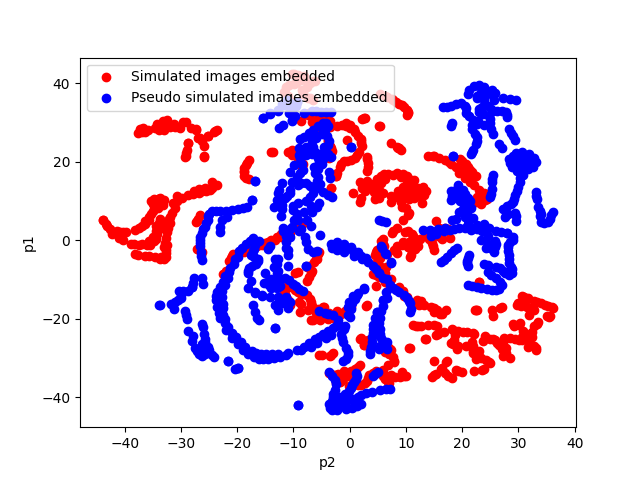
\includegraphics[width=1\textwidth]{experiments/latentr2s.png}
      \caption{Simulated and pseudo simulated images}\label{fig:latentr2s}
  \end{subfigure}%
      \hfill
  \begin{subfigure}{.5\linewidth}
      \centering
      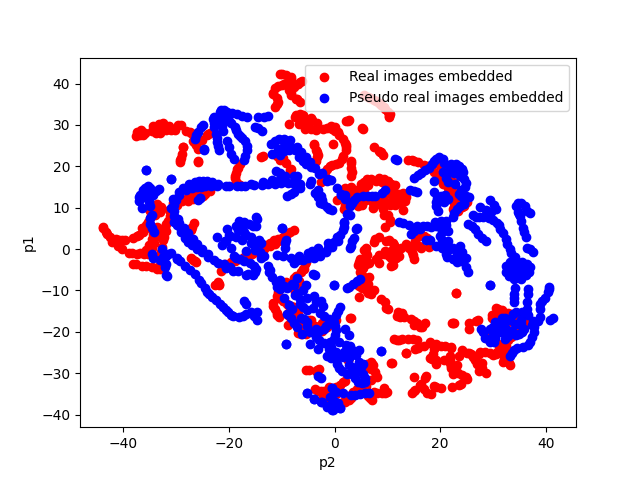
\includegraphics[width=1\textwidth]{experiments/latents2r.png}
      \caption{Real and pseudo real images}\label{fig:latents2r}
  \end{subfigure}
  \caption{Images embedded into the latent space with respectively the simulated and the real VAE.}
  \label{fig:latentpseudo}
\end{figure}
Since the datasets are not aligned we do not except a perfect overlap, instead, the encoder should be able to at least embed similar images in the same region of the space. However, the latent space shows that is not always the case, some regions does overlap but not all off them in both real and simulated dataset. This could lead the trained agent not to respond consistently in similar situations. A further attempt is made by aligning the set of data used through the CycleGAN. Once the the CycleGAN has been used to transform simulated images into pseudo real images, it can be used again to bring them back to pseudo simulated images, resulting in aligned sets. However, notice that the distortion, barely visible before, increases as shown in Figure \ref{fig:examplealigned}.
\begin{figure}[h]
  \centering
  \begin{subfigure}{.33\linewidth}
      \centering
      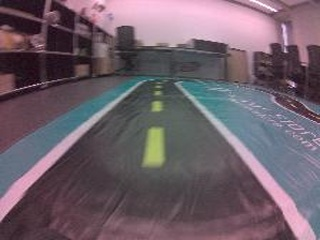
\includegraphics[width=1\textwidth]{experiments/0_.jpg}
      \caption{Real image}\label{fig:real}
  \end{subfigure}%
      \hfill
  \begin{subfigure}{.33\linewidth}
      \centering
      \scalebox{-1}[1]{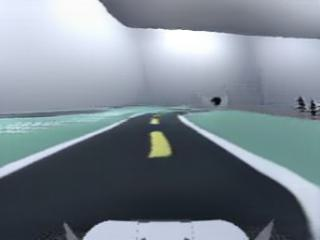
\includegraphics[width=1\textwidth]{experiments/0__.jpg}}
      \caption{Pseudo simulated image}\label{fig:psim}
  \end{subfigure}%
  \hfill
  \begin{subfigure}{.33\linewidth}
    \centering
    \scalebox{-1}[1]{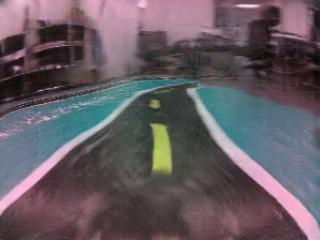
\includegraphics[width=1\textwidth]{experiments/0___.jpg}}
    \caption{Pseudo pseudo real}\label{fig:ppreal}
  \end{subfigure} 
  \caption{Example of using the CycleGan to create an aligned dateset}
  \label{fig:examplealigned}
\end{figure}

\begin{figure}[h]
  \centering
  \begin{subfigure}{.5\linewidth}
      \centering
      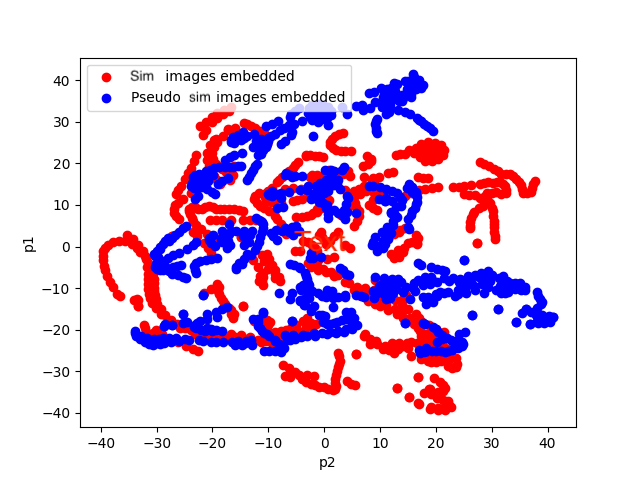
\includegraphics[width=1\textwidth]{experiments/aligned_latentr2s.png}
      \caption{Aligned simulated and pseudo sim images}\label{fig:aligen_latentr2s}
  \end{subfigure}%
      \hfill
  \begin{subfigure}{.5\linewidth}
      \centering
      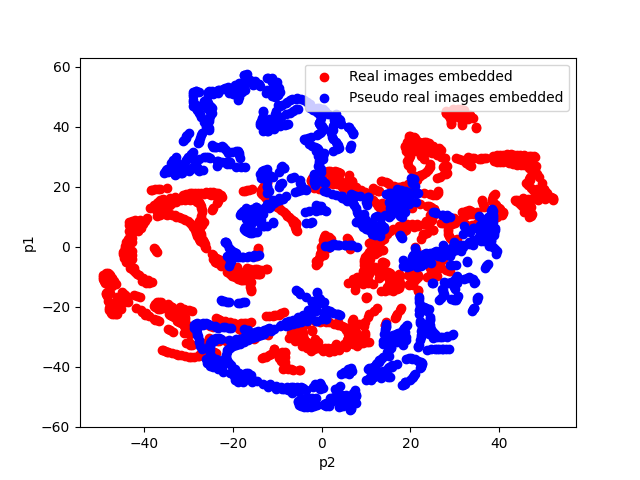
\includegraphics[width=1\textwidth]{experiments/aligned_latents2r.png}
      \caption{Aligned real and pseudo real images}\label{fig:aligen_latents2r}
  \end{subfigure}
  \caption{Aligned images embedded into the latent space with respectively the simulated and the real VAE.}
  \label{fig:latentpseudoaligned}
\end{figure}
Unfortunately, the results do not change enough from the previuos one as shown in Figure \ref{fig:latentpseudoaligned}. Given that the t-SNEe dimensionality reduction may be a cause of our problem, a further investigation is made by checking what are the closest images between the real set and pseudo real set and similarly for the simulation in the latent space. The distance measure used is the Euclidean distance and by looking at them there is some problem, infact there are perfect matches as well as wrong matches as shown in Figures \ref{fig:simdistance} and \ref{fig:realdistance}. This may be the cause of our agent not being able to drive when transferred into another domain, the encoder is not robust enough to compensate little image distortion.

As a final test, we are interested in studying what would be the actions undertakean by the agent on a set of aligned pictures. In particular, we selected a small set of 100 contiguos real pictures of the track and created its \textit{aligned} pseudo real version. We then checked what would be the action of the real agent. As shown in Figure \ref{fig:path_rec}, the results are interesting since most of the times the agent takes the same action on both images, however even a tiny difference can lead the car out of track from which often it is not able to recover.

\begin{figure}[h]
  \begin{center}
    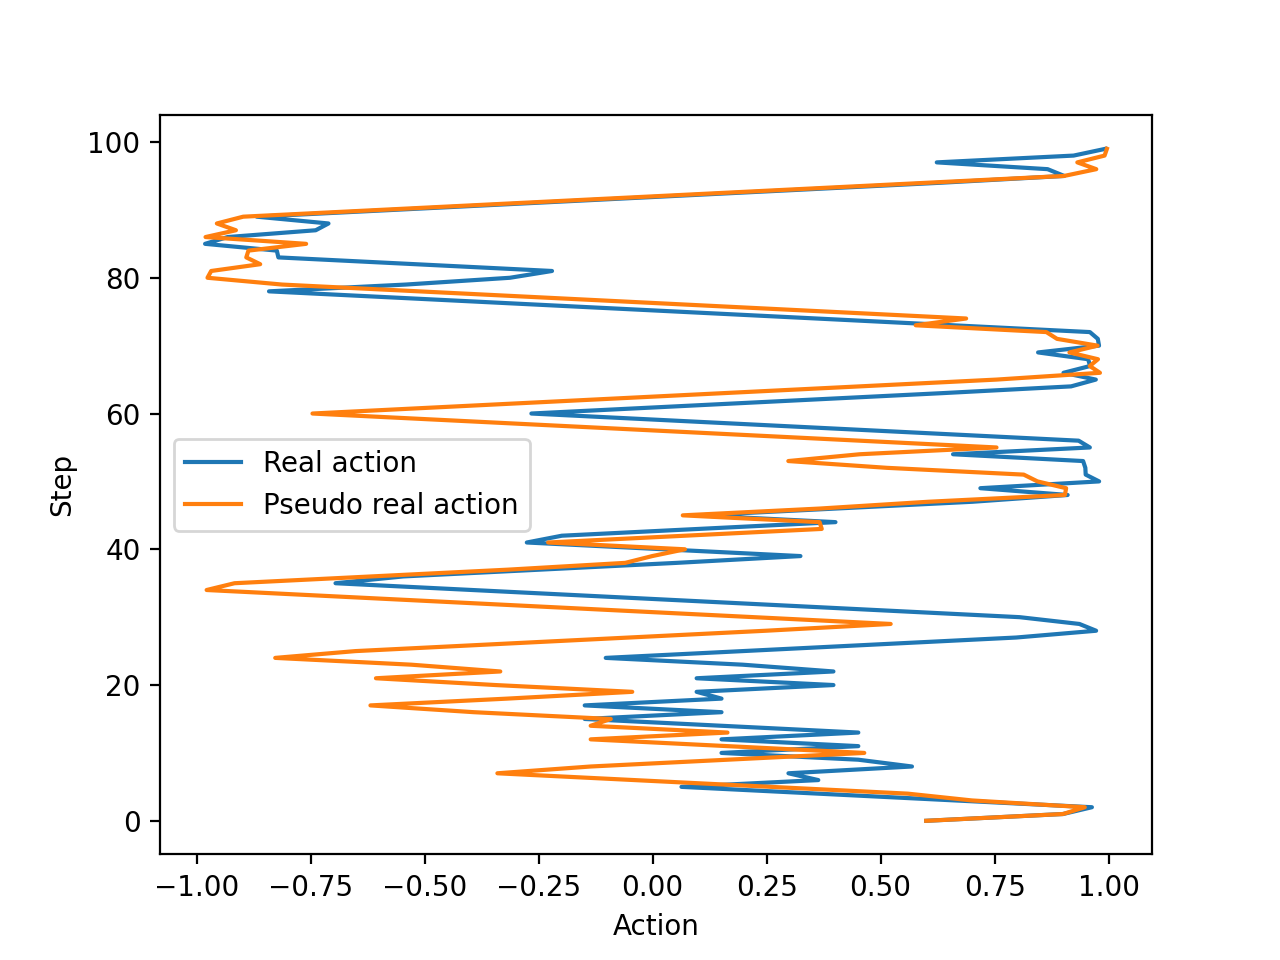
\includegraphics[width=0.60\textwidth]{experiments/path_rec.png}
  \end{center}
  \caption{Real agent's actions on an aligned dataset}
  \label{fig:path_rec}
\end{figure}

\begin{figure}[h]
  \centering
  \begin{subfigure}{.24\linewidth}
      \centering
      \scalebox{-1}[1]{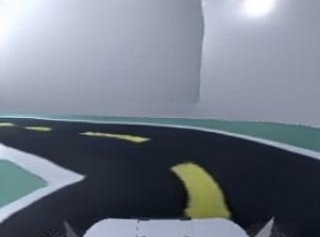
\includegraphics[width=1\textwidth]{experiments/badsimdist1.jpg}}
      \caption{Pseudo simulated}\label{fig:badsimdist1}
  \end{subfigure}%
  \hfill
  \begin{subfigure}{.24\linewidth}
    \centering
    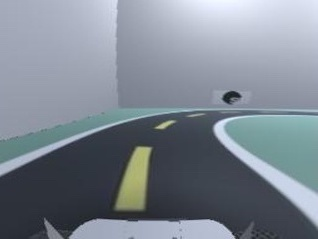
\includegraphics[width=1\textwidth]{experiments/badsimdist2.jpg}
    \caption{Closest simulated}\label{fig:badsimdist2}
  \end{subfigure}%
  \hfill
  \begin{subfigure}{.24\linewidth}
      \centering
      \scalebox{-1}[1]{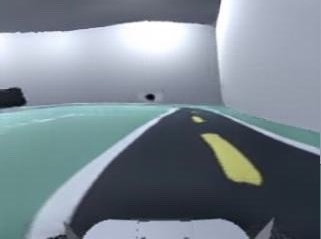
\includegraphics[width=1\textwidth]{experiments/goodsimdist1.jpg}}
      \caption{Pseudo simulated}\label{fig:goodsimdist1}
  \end{subfigure}%
  \hfill
  \begin{subfigure}{.24\linewidth}
    \centering
    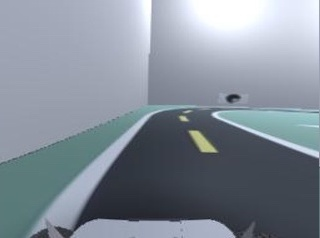
\includegraphics[width=1\textwidth]{experiments/goodsimdist2.jpg}
    \caption{Closest simulated}\label{fig:goodsimdist2}
\end{subfigure}
  \caption{Figures \ref{fig:badsimdist1} and \ref{fig:goodsimdist1} show two pseudo simulated images and Figures \ref{fig:badsimdist2} and \ref{fig:goodsimdist2} respectively the closest match in the simulated set measured with the Euclidean Distance.}
  \label{fig:simdistance}
\end{figure}

\begin{figure}[h]
  \centering
  \begin{subfigure}{.24\linewidth}
      \centering
      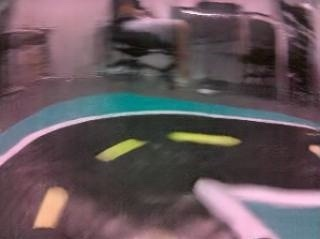
\includegraphics[width=1\textwidth]{experiments/badrealreal1.jpg}
      \caption{Pseudo real}\label{fig:badrealdist1}
  \end{subfigure}%
  \hfill
  \begin{subfigure}{.24\linewidth}
    \centering
    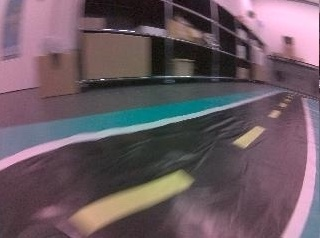
\includegraphics[width=1\textwidth]{experiments/badrealreal2.jpg}
    \caption{Closest real}\label{fig:badrealdist2}
  \end{subfigure}%
  \hfill
  \begin{subfigure}{.24\linewidth}
      \centering
      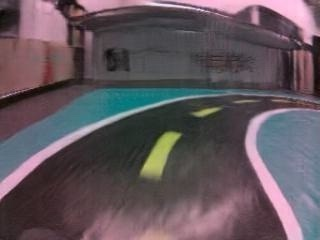
\includegraphics[width=1\textwidth]{experiments/goodrealdist1.jpg}
      \caption{Pseudo real}\label{fig:goodrealdist1}
  \end{subfigure}%
  \hfill
  \begin{subfigure}{.24\linewidth}
    \centering
    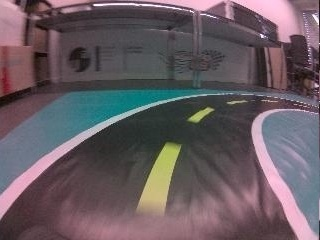
\includegraphics[width=1\textwidth]{experiments/goodrealdist2.jpg}
    \caption{Closest real}\label{fig:goodrealdist2}
\end{subfigure}
  \caption{Figures \ref{fig:badrealdist1} and \ref{fig:goodrealdist1} show two pseudo real images and Figures \ref{fig:badrealdist2} and \ref{fig:goodrealdist2} respectively the closest match in the real set measured with the Euclidean Distance.}
  \label{fig:realdistance}
\end{figure}



